\documentclass[12pt]{article}
\usepackage[utf8]{inputenc}
\usepackage{amsmath,amssymb,hyperref,array,xcolor,multicol,verbatim,mathpazo,algorithm,algpseudocode,enumerate,tikz}
\usepackage[normalem]{ulem}
\usepackage{graphicx}

\newenvironment{problem}[2][Problem]{\begin{trivlist}
\item[\hskip \labelsep {\bfseries #1}\hskip \labelsep {\bfseries #2.}]}{\end{trivlist}}

\begin{document}

%%%% In most cases you won't need to edit anything above this line %%%%

\title{\vspace{-4cm}CS 270 Homework 9}
\author{Neel Gupta} 
\maketitle

\begin{problem}{1}
    In the network $G$ below, the demand values are shown on vertices (supply value if negative). Lower bounds on flow and edge capacities are shown as (lower bound, capacity) for each edge. Determine if there is a feasible circulation in this graph. You need to show all your steps.

    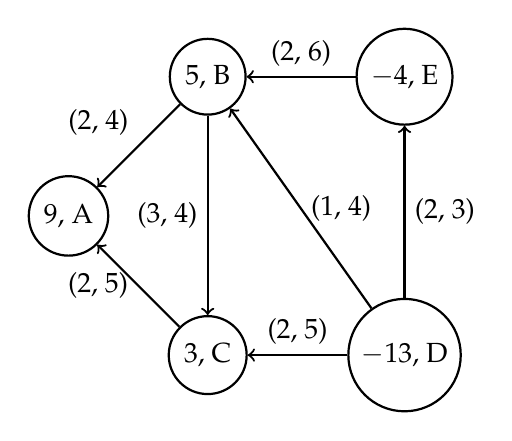
\begin{tikzpicture}[node distance={25mm}, thick, main/.style = {draw, circle}] 
        \node[main] (A) {$9$, A};
        \node[main] (B) [above right of=A] {$5$, B};
        \node[main] (C) [below right of=A] {$3$, C}; 
        \node[main] (D) [right of=C] {$-13$, D}; 
        \node[main] (E) [right of=B] {$-4$, E};
        \draw[->] (D)--(C) node [midway,above] {(2, 5)};
        \draw[->] (C)--(A) node [midway,left] {(2, 5)};
        \draw[->] (B)--(A) node [midway,above left] {(2, 4)};
        \draw[->] (D)--(B) node [midway,right] {(1, 4)};
        \draw[->] (D)--(E) node [midway,right] {(2, 3)};
        \draw[->] (B)--(C) node [midway,left] {(3, 4)};
        \draw[->] (E)--(B) node [midway,above] {(2, 6)};
    \end{tikzpicture} 
    \begin{enumerate}[(a)]
        \item Reduce the Feasible Circulation with Lower Bounds problem to a Feasible Circulation problem without lower bounds.
        \item Reduce the Feasible Circulation problem obtained in part (a) to a Maximum Flow problem in a Flow Network.
        \item Using the solution to the resulting Max Flow problem, explain whether there is a Feasible Circulation in G.
    \end{enumerate}
\end{problem}

\textit{Answer:}\\(a)

Edge (E, B) has lower bound 2, so $E = -4 - 2 =-6$ and $B = 5 + 2 = 7$. 

Capacity left on (B, E) = 6 - 2 = 4.

Edge (D, B) has lower bound 1, so $D = -13-1=-14$ and $B = 7+1=8$.

Capacity left on (D, B) = 4 - 1 = 3.

Edge (D, E) has lower bound 2, so $D = -14 - 2 = -16$ and $E = -6 + 2 =-4$. 

Capacity left on (D, E) = 3 - 2 = 1.

Edge (D, C) has lower bound 2, so $D=-16-2=-18$ and $C = 3+2=5$.

Capacity left on (D, C) = 5 - 2 = 3.

Edge (B, C) has lower bound 3, so $B = 8-3=5$ and $C=5+3=8$. 

Capacity left on (B, C) = 4 - 3 = 1.

Edge (C, A) has lower bound 2, so $C = 8-2=6$ and $A=9+2=11$.

Capacity left on (C, A) = 5 - 2 = 3.

Edge (B, A) has lower bound 2, so $B = 5-2=3$ and $A=11+2 =13$.

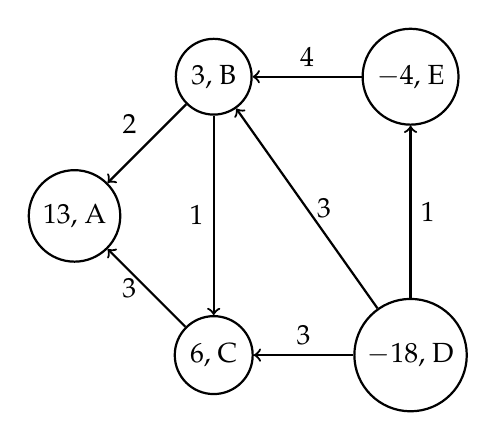
\begin{tikzpicture}[node distance={25mm}, thick, main/.style = {draw, circle}] 
    \node[main] (A) {$13$, A};
    \node[main] (B) [above right of=A] {$3$, B};
    \node[main] (C) [below right of=A] {$6$, C}; 
    \node[main] (D) [right of=C] {$-18$, D}; 
    \node[main] (E) [right of=B] {$-4$, E};
    \draw[->] (D)--(C) node [midway,above] {3};
    \draw[->] (C)--(A) node [midway,left] {3};
    \draw[->] (B)--(A) node [midway,above left] {2};
    \draw[->] (D)--(B) node [midway,right] {3};
    \draw[->] (D)--(E) node [midway,right] {1};
    \draw[->] (B)--(C) node [midway,left] {1};
    \draw[->] (E)--(B) node [midway,above] {4};
\end{tikzpicture} \\ (b)

To reduce the Feasible Circulation problem to the Max Flow problemm, we can add a source node $S$ which connects to all supply nodes and a sink node $T$ which connects to all demand nodes. The supply and demand values will be the edge capacities between these new nodes. Below is the modified graph with the new source and sink nodes.

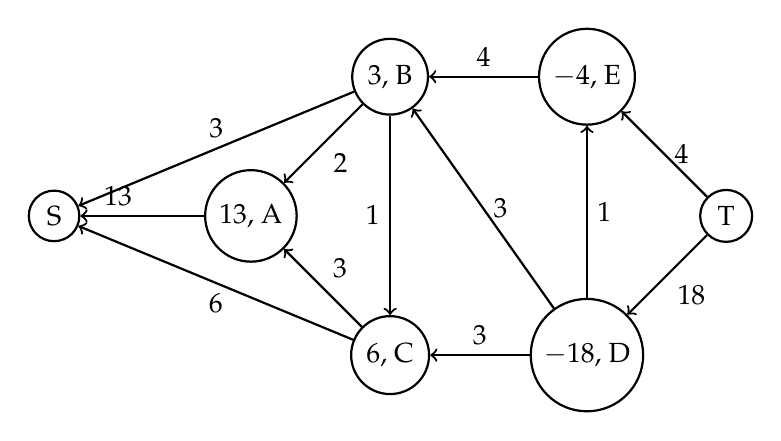
\begin{tikzpicture}[node distance={25mm}, thick, main/.style = {draw, circle}]
    \node[main] (A) {$13$, A};
    \node[main] (B) [above right of=A] {$3$, B};
    \node[main] (C) [below right of=A] {$6$, C};
    \node[main] (D) [right of=C] {$-18$, D};
    \node[main] (E) [right of=B] {$-4$, E};
    \node[main] (S) [left of=A] {S};
    \node[main] (T) [below right of=E] {T};
    \draw[->] (D)--(C) node [midway,above] {3};
    \draw[->] (C)--(A) node [midway,above right] {3};
    \draw[->] (B)--(A) node [midway,below right] {2};
    \draw[->] (D)--(B) node [midway,right] {3};
    \draw[->] (D)--(E) node [midway,right] {1};
    \draw[->] (B)--(C) node [midway,left] {1};
    \draw[->] (E)--(B) node [midway,above] {4};
    \draw[->] (A)--(S) node [midway,above left] {13};
    \draw[->] (B)--(S) node [midway,above] {3};
    \draw[->] (C)--(S) node [midway,below] {6};
    \draw[->] (T)--(D) node [midway,below right] {18};
    \draw[->] (T)--(E) node [midway,right] {4};
\end{tikzpicture} \\ (c)

After running either Ford-Fulkerson or Edmonds-Karp, if we find a max-flow which is equal to the total demand out and the total supply then there is a feasible circulation with lower bounds. There is 22 out as well as there is 22 in, so there is a feasible circulation for the given supplies and demands with the lower bounds in place.

\begin{problem}{2}
    In a standard minimum $s-t$ cut problem, we assume that all capacities are nonnegative; allowing an arbitrary set of positive and negative capacities results in a problem that is computationally much more difficult. However, as we'll see here, it is possible to relax the nonnegativity requirement a little and still have a problem that can be solved in polynomial time.

    Let $G=(V,E)$ be a directed graph, with source $s \in V$, $t \in V$, and edge capacities ${c_e}$. Suppose that for every edge $e$ that has neither $s$ not $t$ as an endpoint, we have $c_e \geq 0$. Thus $c_e$ can be negative for edeges $e$ that have at least one end equal to either $s$ or $t$. Give a polynomial-time algorithm to find an $s-t$ cut of minimum value in such a graph. (Despite the new nonnegativity requirements, we still define the value of an $s-t$ cut $(A,B)$ to be the sum of the capacities of all edges $e$ for which the tail of $e$ is in $A$ and the head of $e$ is in $B$.)
\end{problem}

\textit{Answer:}

\begin{enumerate}[1.]
    \item Create a new graph $G'=(V', E')$ as a copy of the original graph $G$. Add an additional source $S'$ and additional sink $T'$.
    \item For every edge $e:=(s,v)$ with a negative edge capacity $c_e$ in the original graph $G$, add an edge $e':=(s',v)$ with capacity $-c_e$ in $G'$. Also, add an edge $(s,v)$ with capacity 0.
    \item For every edge $e:=(v,t)$ with a negative edge capacity $c_e$ in the original graph $G$, add an edge $e':=(v,t')$ with capacity $-c_e$ in $G'$. Also, add an edge $(v,t)$ with capacity 0.
    \item Run Edmonds-Karp algorithm on $G'$ to find a minimum $s'-t'$ cut say $(A', B')$.
    \item Map the cut $(A', B')$ back to the original graph $G$. Create sets $A$ and $B$ by removing $s'$ and $t'$ from $A'$ and $B'$, respectively. The resulting $s-t$ cut $(A, B)$ in $G$ corresponds to the minimum $s-t$ cut in $G'$ with the relaxed non-negativity requirements.
\end{enumerate}

Consider using the Edmonds-Karp algorithm to find the max-flow in the constructed flow network. The time complexity of Edmonds-Karp is $O(|V| \cdot |E|^2)$, where $|V|$ is the number of vertices and $|E|$ is the number of edges in the graph. The algorithm has up to $O(E)$ operations, so the overall runtime is $O(|V| \cdot |E|^2)$ which means the runtime is polynomial.

\begin{problem}{3}
    At a dinner party, there are $n$ families $\{a_1, a_2, ..., a_n\}$ and $m$ tables $\{b_1,b_2,...,b_m\}$. The $i$th family $a_i$ has $g_i$ members and the $j$th table $b_j$ has $h_j$ seats. Everyone is interested in making new friends and the dinner party planner wants to seat people such that no two members of the same family are seated in the same table. Design an algorithm that decies if there exists a seating assignment such that everyone is seated and no two members of the same family are seated at the same table.
\end{problem}

\textit{Answer: }

To solve this problem, you can model it as a bipartite matching problem and then apply a maximum cardinality bipartite matching algorithm, such as the Hopcroft-Karp algorithm.

\begin{enumerate}[1.]
    \item Create a bipartite graph $G = (U, V, E)$, where $U$ represents families and $V$ represents tables.
    \item Add a node $u_i$ in $U$ for each family $a_i$, and a node $v_j$ in $V$ for each table $b_j$.
    \item Connect $u_i$ to $v_j$ with an edge $e_{ij}$ if it's possible to seat a member of family $a_i$ at table $b_j$. Since no two members of the same family can be seated at the same table, each family node $u_i$ should have a maximum degree of min($g_i$, $m$).
    \item Run the Hopcroft-Karp algorithm on the bipartite graph $G$ to find the maximum cardinality matching $M$.
    \item If the size of the maximum cardinality matching or $|M|$ is equal to the total number of family members (i.e., the sum of $g_i$ for all families), then there exists a seating assignment such that everyone is seated, and no two members of the same family are seated at the same table. Otherwise, it's not possible to satisfy the given conditions.
\end{enumerate}

The Hopcroft-Karp algorithm runs in $O(E \sqrt{V})$, so this is an efficient polynomial time solution to find whether a valid seating arrangement exists.

\begin{problem}{4}
    Due to large-scale flooding in a region, paramedics have identified a set of $n$ injured people distributed across the region who need to be rushed to hospitals. There are $k$ hospitals in the region, and each of the $n$ people need to be brought to a hospital that is within a half-hour's drive to their current location. (So different patients will be able to be served by different hospitals depending upon the patients' locations.) However, overloading one hospital with too many patients at the same time is undesirable, so we would like to distribute patients as evenly as possible across all hospitals. So the paramedics (or a centralized service advising the paramedics) would like to work out whether they can choose a hospital for each of the injured people in such a way that each hospital recieves at most $(n/k+1)$
    \begin{enumerate}[(a)]
        \item Describe a procedure that takes the given information about the patients' locations (hence specifying which hospital each patient could go to) and determines whether a balanced allocation of patients is possible (i.e. each hospital recieves at most $(n/k+1)$ patients)
        \item Provide proof of correctness for your procedure.
        \item What is the asymptotic running time of your procedure (in terms of $n$ and $k$)?
    \end{enumerate}
\end{problem}

\textit{Answer:} 
\\ (a) To determine whether a balanced allocation of patients is possible, we can model the problem as a maximum flow problem and solve it using a maximum flow algorithm, such as the Edmonds-Karp algorithm.

\begin{enumerate}[1.]
    \item Create a directed graph $G=(V,E)$ with a source node $s$ and a sink node $t$.
    \item Add a node $p_i$ to $V$ for each patient $i$, and a node $h_j$ in $V$ for each hospital $j$.
    \item Connect $s$ to each $p_i$ with an edge with capacity 1.
    \item For each patient $i$, connect the patient node $p_i$ to the hospital node $h_j$ with an edge with capacity 1 if hospital $j$ is within a half-hour's drive from patient $i$.
    \item Connect each hospital node $h_j$ to $t$ with an edge with capacity $(n/k+1)$.
    \item Run Edmonds-Karp on the directed graph $G$ to find max-flow.
    \item If the maximum flow found is equal to $n$, then a balanced allocation of patients is possible. Otherwise, a balanced allocation is not possible.
\end{enumerate}
(b)
\textbf{Forward direction:} If the max-flow is $n$, the team can have all the $n$ people.

\begin{enumerate}
\item If the max-flow is $n$, there is a unit flow from each person to a single hospital.
\item Since this max-flow is a valid flow, every hospital has a valid number of people.
\item Thus, the team can have all the $n$ people.
\end{enumerate}

\textbf{Backward direction:} If the team can have all the $n$ people, the max-flow is $n$.

\begin{enumerate}
\item If the team can have all the $n$ people, hospital nodes can accept all the $n$ flow.
\item Thus, the max-flow is at least $n$.
\item Also, the max-flow cannot be more than $n$ because there are only $n$ edges from the source node $s$. Thus, the max-flow is $n$.
\end{enumerate}

Therefore, the max-flow algorithm correctly determines whether a balanced allocation of patients is possible by checking if the max-flow is equal to $n$. If the max-flow is equal to $n$, all patients can be assigned to hospitals while maintaining the balanced allocation.
\\(c)

Consider using the Edmonds-Karp algorithm to find the max-flow in the constructed flow network. The time complexity of Edmonds-Karp is $O(|V| \cdot |E|^2)$, where $|V|$ is the number of vertices and $|E|$ is the number of edges in the graph.

In our constructed graph, we have $n + k + 2$ vertices ($n$ patients, $k$ hospitals, the source $s$, and the sink $t$) and $n + k + nk$ edges (each person is connected to at most $k$ hospitals, $n$ edges from the source, and $k$ edges to the sink). Therefore, the time complexity is:
$$
    O((n+k+2)\cdot(n+k+nk)^2)
$$
Asymptotically, this becomes:
$$
O(nk^3)
$$
So the running time of our procedure is $O(nk^3)$.


\end{document}